\chapter{Aquisição de Dados e Treinamento Offline}
O projeto foi dividido em 4 etapas: A confecção e treinamento da Tiny-CNN multiclasse utilizando Python e Keras, a implementação do modelo matemático da CNN em Verilog, dividido em módulos de convolução 3×3 com ReLU (4 filtros), Max Pooling 2×2, Flatten e camada Densa 900×19, a construção da lógica de transmissão via UART da imagem obtida para a FPGA, assim como lógica de a transmissão de imagem exibida em um monitor VGA, e, por fim, a confecção de sprites identificadores dos integrantes e a integração de todos os módulos e seu respectivo teste de funcionamento na FPGA DE2-115.

\section{Confecção e treinamento da Rede Neural Convolucional (CNN)}
O foco desta etapa foi a criação de um pipeline robusto para aquisição de dados, treinamento de uma Tiny-CNN otimizada e a exportação dos parâmetros quantizados para o hardware. O dataset foi projetado para um problema de classificação multiclasse com 19 classes: Classe 0 (Desconhecidos) e Classes 1–18 (Membros autorizados).

\subsection{Classes de 1 a 18: Autorizados (Equipe)}
As imagens foram extraídas de vídeos .mp4 ou pastas, utilizando o algoritmo Haar Cascade com scale Factor 1.2 para detecção facial, e houve a implementação do CLAHE (Contrast Limited Adaptive Histogram Equalization) para garantir o reconhecimento sob diferentes condições de luz e sombras. Para atingir a meta de 400 imagens por integrante, houve a aplicação de técnicas de aumento de dados incluindo rotação leve (-15° a 15°), variações de zoom (0.9x a 1.1x), espelhamento horizontal e ajustes de brilho.

Classe 0: Desconhecidos (Unknowns)
Para minimizar falsos positivos, a Classe 0 foi expandida para garantir maior diversidade, logo tivemos a integração do LFW (Labeled Faces in the Wild) via kagglehub e do UCF Selfie-dataset, utilizando de uma proporção de 5:1 (Desconhecidos:Autorizados) para cobrir a variabilidade do rosto humano. Foram aplicadas então as mesmas técnicas de aumento de dados (rotação/zoom) na Classe 0 para garantir a invariância de identidade, além da inclusão de 300 imagens sintéticas (paredes e ruído) para evitar autorizações baseadas em texturas de fundo.

\begin{figure}[H]
    \centering
    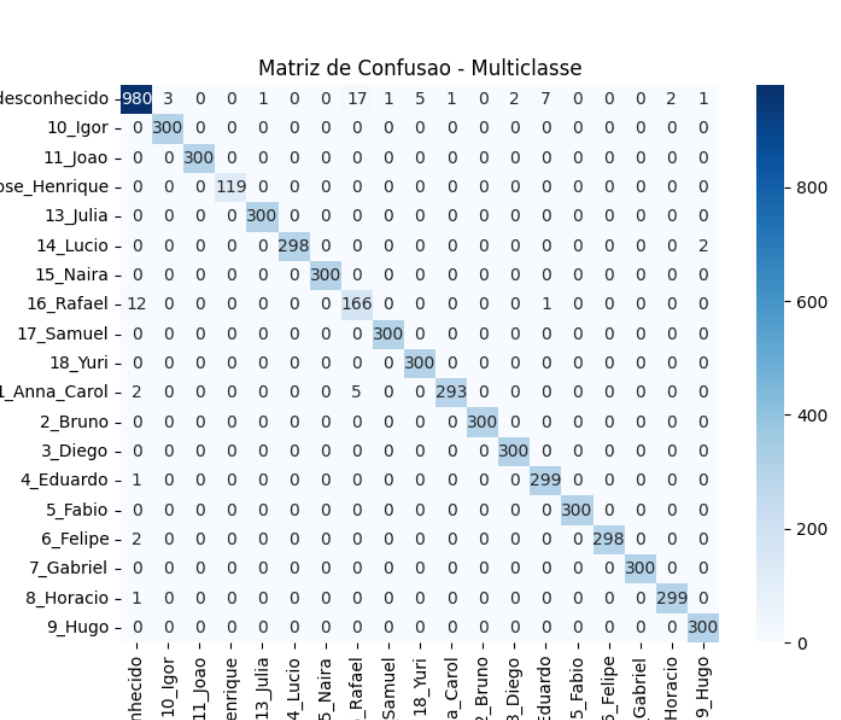
\includegraphics[width=0.8\linewidth]{imagens/image6.png}
    \caption{Matriz de Confusão durante o teste}
    \label{fig1}
\end{figure}

\section{Implementação}
A rede foi projetada para ser leve (Tiny-CNN) visando a implementação em blocos de memória M9K da FPGA, equilibrando capacidade discriminativa e custo computacional compatível com o Cyclone IV EP4CE115F29C7.
A arquitetura segue o pipeline: Entrada 32×32 (grayscale, Q1.7) → Conv2D (4 filtros 3×3, acumuladores 20 bits) → ReLU (combinacional) → Max-Pooling 2×2 → Dropout → Dense (19 classes) → Softmax. 

A escolha de apenas 4 filtros convolucionais não é arbitrária — ela resulta diretamente da restrição de hardware: cada filtro ocupa um sub-bloco M9K dedicado para armazenar seus 900 pesos densos correspondentes, e o Cyclone IV dispõe de 432 blocos M9K, dos quais 19 são consumidos pelos pesos da camada densa (um por classe) e outros são reservados para framebuffer e line buffer.

A busca de hiperparâmetros foi conduzida com Keras Tuner (Hyperband) otimizando simultaneamente a taxa de Dropout (0,2 a 0,5), a Learning Rate e a regularização L2. A escolha do Hyperband sobre o grid search convencional foi motivada pela relação classes/parâmetros: com 19 classes e dataset balanceado artificialmente, o espaço de hiperparâmetros relevante é estreito e o Hyperband converge para ele com menos avaliações completas.

A regularização L2 cumpre papel duplo no projeto: além de reduzir overfitting, ela penaliza pesos de grande magnitude durante o treino, o que reduz diretamente o erro de arredondamento introduzido pela quantização posterior para Q1.7 — pesos próximos de zero perdem menos informação relativa ao serem truncados para 8 bits do que pesos de grande amplitude.

O Custom Loss Weighting aplicou peso 1,0 à Classe 0 (Desconhecido) e 4,0 às classes de membros autorizados (1–18), refletindo a assimetria de custo do problema: uma falsa negação — negar acesso a um membro autorizado — é operacionalmente mais custosa do que um falso positivo para a classe de rejeição. O treinamento foi conduzido com EarlyStopping com paciência de 15 épocas, suficiente para absorver platôs de validação comuns em datasets pequenos com augmentation agressivo.

\begin{figure}[H]
    \centering
    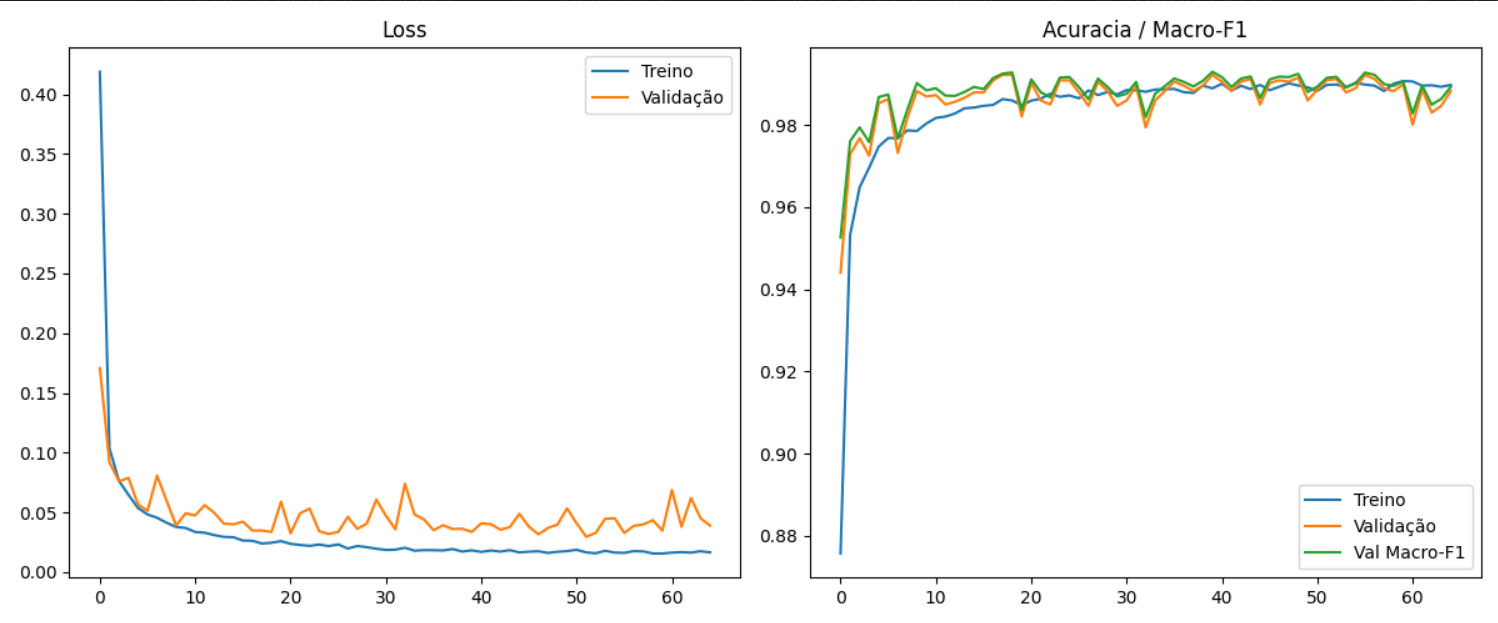
\includegraphics[width=1\linewidth]{imagens/image4.png}
    \caption{Matriz de Confusão durante o teste}
    \label{fig2}
\end{figure}

\section{Inferência e Validação}
O sistema utiliza um script de validação (\texttt{inference\_webcam.py}) sincronizado com o pipeline de hardware. Aplica-se o mesmo pré-processamento (CLAHE, Padding de 15\%, Redimensionamento) utilizado no treino, e ocorre então a exibição da ``Visão da CNN'' (32x32) para validação da qualidade da entrada em tempo real. 

\subsection{Métricas de Treinamento}

Durante a fase de treinamento do modelo, as seguintes métricas globais foram obtidas, evidenciando a capacidade de aprendizado e convergência da rede:

\begin{itemize}
    \item \textbf{AUC OvR (macro):} 0.9999
    \item \textbf{Macro-F1:} 0.9901
    \item \textbf{Balanced Accuracy:} 0.9918
    \item \textbf{Recall da classe desconhecido (negar invasor):} 0.9608
    \item \textbf{Recall macro dos alunos autorizados:} 0.9936
\end{itemize}

\subsection{Métricas de Teste e Relatório de Classificação}

Os resultados da avaliação multiclasse do são dados a seguir:

\begin{itemize}
    \item \textbf{AUC OvR (macro):} 0.9999
    \item \textbf{Macro-F1:} 0.9901
    \item \textbf{Balanced Accuracy:} 0.9918
    \item \textbf{Recall da classe desconhecido (negar invasor):} 0.9608
    \item \textbf{Recall macro dos alunos autorizados:} 0.9936
\end{itemize}

A Tabela \ref{tab:relatorio_classificacao} detalha as métricas de precisão, revocação (\textit{recall}) e pontuação F1 para cada classe individualmente, bem como as médias globais do sistema.

\begin{table}[H]
\centering
\caption{Relatório de Classificação}
\label{tab:relatorio_classificacao}
\begin{tabular}{l c c c c}
\toprule
\textbf{Classe} & \textbf{Precision} & \textbf{Recall} & \textbf{F1-score} & \textbf{Support} \\
\midrule
0\_desconhecido    & 0.98 & 0.96 & 0.97 & 1020 \\
10\_Igor           & 0.99 & 1.00 & 1.00 & 300  \\
11\_Joao           & 1.00 & 1.00 & 1.00 & 300  \\
12\_Jose\_Henrique & 1.00 & 1.00 & 1.00 & 119  \\
13\_Julia          & 1.00 & 1.00 & 1.00 & 300  \\
14\_Lucio          & 1.00 & 0.99 & 1.00 & 300  \\
15\_Naira          & 1.00 & 1.00 & 1.00 & 300  \\
16\_Rafael         & 0.88 & 0.93 & 0.90 & 179  \\
17\_Samuel         & 1.00 & 1.00 & 1.00 & 300  \\
18\_Yuri           & 0.98 & 1.00 & 0.99 & 300  \\
1\_Anna\_Carol     & 1.00 & 0.98 & 0.99 & 300  \\
2\_Bruno           & 1.00 & 1.00 & 1.00 & 300  \\
3\_Diego           & 0.99 & 1.00 & 1.00 & 300  \\
4\_Eduardo         & 0.97 & 1.00 & 0.99 & 300  \\
5\_Fabio           & 1.00 & 1.00 & 1.00 & 300  \\
6\_Felipe          & 1.00 & 0.99 & 1.00 & 300  \\
7\_Gabriel         & 1.00 & 1.00 & 1.00 & 300  \\
8\_Horacio         & 0.99 & 1.00 & 1.00 & 300  \\
9\_Hugo            & 0.99 & 1.00 & 1.00 & 300  \\
\midrule
\textbf{accuracy}     &      &      & 0.99 & 6118 \\
\textbf{macro avg}    & 0.99 & 0.99 & 0.99 & 6118 \\
\textbf{weighted avg} & 0.99 & 0.99 & 0.99 & 6118 \\
\bottomrule
\end{tabular}
\end{table}

\section{Quantização e Exportação (.MIF)}
Os pesos são convertidos de ponto flutuante para Ponto Fixo (Q1.7) para execução em hardware de 8 bits, seguindo a lógica de multiplicação por 128 (27) e arredondamento para o intervalo de -128 a 127. Então, são gerados os ficheiros .mif formatados para os blocos de memória M9K do Intel Quartus Prime.
